\subsection{Peripherie}

Im folgenden werden die verschiedenen benutzten Peripherien erläutert. Diese beziehen sich jedoch primär auf die Funktionen des STM32, da diese
dort intensiver Nutzung unterliegen, während die einzig genutzten Funktionalitäten des ESP8266 seine WLAN- und UART-Schnittstelle sind,
welche durch das Arduino-Framework verschleiert werden.

\subsubsection{UART/USART}

Der STM32F103 verfügt über drei \ac{USART}-Schnittstellen, welche jedoch auch als \ac{UART} genutzt werden können \citep{STM32_Datasheet}.
Die dabei genutzten Spannungspegel entsprechen hierbei die der TTL-Logik \citep{STM32_Datasheet}.

\smallskip

Die Einheiten verfügen unter anderem auch über Idle-Line Detection (\textit{Erkennung von Kommunikationsstops}), Duplex und Hardware Flow 
Control \citep{STM32_Ref}.




\subsubsection{DMA}

\begin{wrapfigure}{r}{0.35\textwidth}
    % \begin{figure}[h]
     \vspace{-\baselineskip}
         \centering
         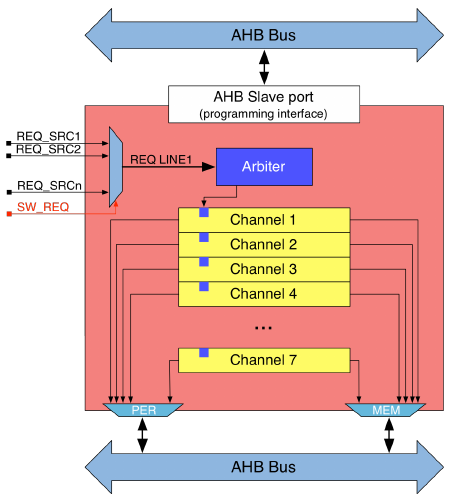
\includegraphics[scale=0.3]{Pictures/dma_channel.png}
         \caption{\textit{DMA \citep{MasteringSTM}}}
         \label{img:DMA_Controller}
    % \end{figure}
 \end{wrapfigure}

Der \acl{DMA} Controller ist eine dedizierte Hardwareeinheit, welche das direkte Schreiben von Daten in den Speicher des \ac{uC} erlaubt, ohne dass dafür Instruktionen durch den Prozessor
ausgeführt werden müssen. Die unterstützten Peripherien sind Timer, \acs{ADC}, \acs{SPI}, \acs{I2C} und \acs{UART} \citep{STM32_Datasheet}.

\smallskip

Daten können von Speicherort zu Speicherort, von einer Peripherie zu einem Speicherort oder von einem Speicherort zu einer Peripherie transferiert werden.
Der STM32F103 verfügt über sieben \ac{DMA}-Kanäle.

\smallskip

Durch die Nutzung von \ac{DMA} wird der Prozessor entlastet, da er dann nicht mit der Übertragung von Daten blockiert wird. Die Daten werden 
über eine interne Busmatrix direkt übertragen \citep{MasteringSTM}.

\smallskip

Abbildung \ref{img:DMA_Controller} zeigt den Aufbau eines einzelnen Controllers. Der Nutzer kann den verschiedenen Kanälen,
die jeweils mit einer Peripherieeinheit verknüpft werden können, Prioritäten zuweisen. Die Priorität der DMA-Controller werden durch den Arbiter verwaltet.
Der \ac{DMA} ist über den \ac{AHB-Bus}, mit den 
Peripherieeinheiten und dem Speicher des \ac{uC} verknüpft \citep{MasteringSTM}.

\smallskip

Der \ac{DMA}-Controller verfügt über einen Slave-Port. Mittels dieses Anschlusses lässt sich der \ac{DMA}-Controller konfigurieren \citep{MasteringSTM}.

\newpage

\subsubsection{ADC}

Ein \acs{ADC} ermöglicht die Konversion von analogen Signalen in digitale Werte, um diese anschließend durch den \ac{uC} weiterzuverarbeiten. 
Der \ac{ADC} des STM32F103 hat eine Auflösung von 12-Bit bei bis zu 16 Kanälen und arbeitet nach dem Prinzip der sukzessiven Approximation \citep{STM32_Datasheet}.

\smallskip


\begin{figure}[h]
     \vspace{-\baselineskip}
         \centering
         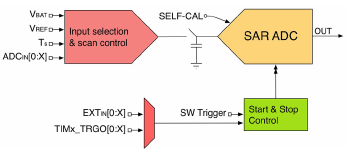
\includegraphics[scale=0.6]{Pictures/adc.png}
         \caption{\textit{Aufbau \citep{MasteringSTM}}}
         \label{img:ADC}
\end{figure}


Es ist möglich, den \ac{ADC} automatisch zu kalibrieren und ihn entweder per Software-Trigger, Timer oder externen Interrupt zu starten. 
In Abbildung \ref{img:ADC} ist der vereinfachte Aufbau des \ac{ADC} abgebildet.

\smallskip 

Der \ac{ADC} verfügt über verschiedene Betriebsmodi \citep{STM32_Ref}:
\begin{itemize}
    \item Single Mode 
    \item Continuous Mode
    \item Discontinuous Mode
\end{itemize}

Im Single Mode wird eine Konversion durchgeführt, während im Continuous Mode ständig weitere Konversionen durchgeführt werden. Im Discontinuous Mode
wird die nächste Konversion durchgeführt, sobald ein benutzerdefinierter Trigger ausgelöst wird. Es ist im (Dis-)Continuous Mode möglich, bei 
jeder Konversion einen anderen Kanal des \ac{ADC} anzusprechen.

\newpage

\subsubsection{GPIO}

Der STM32F103 besitzt diverse \acs{GPIO}. Mit Hilfe dieser Ein- und Ausgänge können Signale ein- oder ausgegeben werden. Es ist möglich,
den Anschlüssen interne Pull-Up oder Pull-Down Widerstände zuzuweisen \citep{STM32_Datasheet}. Ausgänge können entweder als Push-Pull oder Open-Drain
konfiguriert werden \citep{STM32_Ref}.

\smallskip

Die Eingänge können,je nach anliegendem Signal, Interrupts auslösen \citep{STM32_Ref}:
\begin{itemize}
    \item Steigende Flanke
    \item Fallende Flanke
    \item Steigende oder Fallende Flanke
\end{itemize}

Die interne Beschaltung der \ac{GPIO} ist Abb. \ref{img:GPIO} zu entnehmen.

\vspace{0.5cm}

\begin{figure}[h]
    \vspace{-\baselineskip}
        \centering
        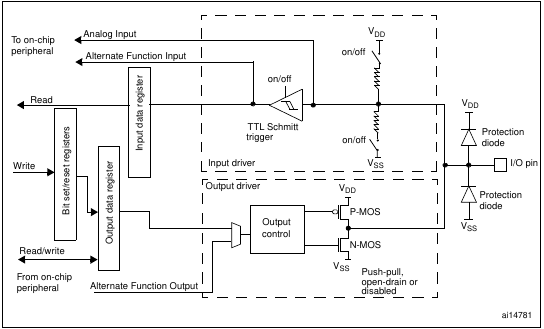
\includegraphics[scale=0.6]{Pictures/gpio.png}
        \caption{\textit{Beschaltung \citep{STM32_Ref}}}
        \label{img:GPIO}
\end{figure}

\newpage


\subsubsection{Timer}
\label{subsub: Timer}

Die Timer des STM32F103 teilen sich, wie in Abb. \ref{img:Timer} zu sehen, in zwei Gruppen auf:

\vspace{0.5cm}
\begin{figure}[h]
    \vspace{-\baselineskip}
        \centering
        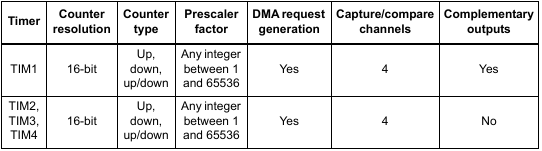
\includegraphics[scale=0.6]{Pictures/timer.png}
        \caption{\textit{Timer \citep{STM32_Datasheet}}}
        \label{img:Timer}
\end{figure}

TIM1 ist ein Advanced-Control Timer, während TIM2,TIM3 und TIM4 General-Purpose Timer sind. 

Advanced-Control Timer implementieren erweiterte Funktionen, wie z.B. dreiphasige Pulsweitenmodulation oder programmierbare 
Totzeiten\citep{STM32_Datasheet}. 

\smallskip

Abgesehen von den bereits vorgestellten Timern stehen zwei Watchdog-Timer sowie ein SysTick-Timer zur Verfügung. Der SysTick-Timer wird einerseits genutzt,
um ein Real-Time Operating System auf dem STM32F103 zu realisieren und andererseits, um 
dem Hardware Abstraction Layer des STM32F103 eine Zeitkonstante zu geben. Er kann auch als simpler Timer benutzt wird, da er jede
ms aktualisiert wird.

\smallskip

Watchdog-Timer werden genutzt, um abnormale Systemzustände zu erkennen. Ein Beispiel hierfür ist das Festhängen in spezifischen Codeabschnitten.



